\begin{figure}
    \centering
    \scalebox{.99}{
    \begin{tikzpicture}[
        node distance=1.2cm and 2cm,
        data/.style={rectangle, draw, dashed, minimum width=2.5cm, minimum height=0.9cm, align=center, font=\small},
        arrow/.style={->, thick},
        interp/.style={->, thick},
        operation/.style={font=\footnotesize, midway, above},
        operationside/.style={font=\footnotesize, midway, right},
        operationleft/.style={font=\footnotesize, midway, left},
        bigbox/.style={draw, thick, rounded corners, inner sep=0.3cm},
        impl/.style={font=\tiny, text=gray}
    ]
        % Slice compiler pipeline (horizontal inside the box)
        \node[data] (ast) {AST\\{\tiny\texttt{expr}}};
        \node[data, right=of ast] (tast) {Typed AST\\{\tiny\texttt{texpr}}};
        \node[data, right=of tast] (dast) {Discretized\\{\tiny \texttt{expr}}};
        
        % Input above AST
        \node[data, above=1.5cm of ast] (input) {\texttt{.slice} file\\{\footnotesize continuous program}};
        
        % Slice compiler box
        \node[bigbox, fit=(ast)(tast)(dast), inner sep=0.5cm, label=above:{\textbf{\Slice{} Discretizer}}] (slicebox) {};
        
        % ast.ml in top right corner of compiler box
        \node[impl] at ($(slicebox.south) + (0.0,0.25)$) {ast.ml, utils.ml, pretty.ml};
        
        % Output below dast
        \node[data, below=1.55cm of dast] (dice) {\texttt{.dice} / \texttt{.rkt} / \\\texttt{.tra} / \texttt{.lab} file\\{\footnotesize discrete program}};
        
        % Dice engine result to the left of dice output
        \node[data, left=2.6cm of dice] (output) {Probability\\Distribution};
        
        % Arrows with operations
        % Input to compiler
        \draw[arrow] (input) -- node[operationside, yshift=5mm, xshift=1mm] {Parse} (ast);
        \node[impl, align=center] at ($(input)!0.5!(ast) + (0.6,0.1)$) {parser.mly\\lexer.mll};
        
        % Inside compiler
        \draw[arrow] (ast) -- node[operation] {Type Infer} (tast);
        \node[impl, align=center] at ($(ast)!0.5!(tast) + (0,-0.4)$) {inference.ml\\lats.ml(i)};
    
        \draw[arrow] (tast) -- node[operation] {Discretize} (dast);
        \node[impl, align=center] at ($(tast)!0.5!(dast) + (0,-0.4)$) {discretization.ml\\distributions.ml};
        
        % Compiler to output
        \draw[arrow] (dast) -- node[operationside, yshift=-1mm] {Convert} (dice);
        \node[impl, align=center] at ($(dast)!0.5!(dice) + (1.3,-0.4)$) {to\_\{dice,roulette,mc\}.ml};
        
        % Backend engine - horizontal arrow from dice to output
        \draw[arrow] (dice.west) -- node[operation, align=center] {Dice / Roulette / \\ Storm Engine} (output.east);
        \node[impl, align=center] at ($(dice)!0.5!(output) + (0,-0.4)$) {BDD + WMC / \\ DTMC model checking};
        
        % Interpreter arrows
        \draw[interp] (ast.south) .. controls +(0,-0.5) and +(0,1) .. 
            node[operationleft, font=\footnotesize, align=center, yshift=-5mm, xshift=8mm] {Interpreter\\[-1mm]{\tiny \textcolor{gray}{interp.ml}}} (output.north);
        \draw[interp] (dast.south) .. controls +(0,-0.5) and +(0,1) .. (output.north);
    \end{tikzpicture}}
    \caption{Pipeline for exact discretization: typed \Slice{} programs are transformed into semantically equivalent discrete programs, then evaluated by discrete exact-inference engines. The transformation stage (type inference + discretization) is backend-agnostic; \Dice{}, \Roulette{}, and \Storm{} are current examples of target backends.}
    \label{fig:architecture}
\end{figure}


\section{Slice by Example}\label{sec:examples}
% We illustrate the main \Slice{} constructs—conditionals, local bindings, functions, sampling, and conditioning—through a set of small programs; Appendix~\ref{ap:mot} contains additional examples.

% For readability, we use \flip() as a shorthand for \uniform(0,1) < 0.5, which represents a fair coin flip that returns true or false with equal probability. A cut $\clt{c}$ refers to any constant $c$ that appears in a comparison such as $x < c$, where $c$ divides the real line $\R$ into two intervals: $(-\infty, c)$ and $[c, +\infty)$. When $x$ is compared to several constants, these comparisons introduce a set of cuts $\clt{c_1}, \ldots, \clt{c_n}$, which partitions $\R$ into $n+1$ contiguous intervals $(-\infty, c_1), [c_1,c_2), \ldots, [c_{n-1}, c_n), [c_n, +\infty)$.


% \subsection{Simple Branching on a Uniform Distribution}\label{sec:examples:1}

% We start with a basic example that illustrates the core idea of \Slice{}. 
We can model a fair coin flip by comparing a uniform sample to $0.5$:

\begin{lstlisting}[aboveskip=1em,belowskip=1em]
    uniform(0,1) < 0.5
\end{lstlisting}

% \noindent 

Instead of sampling a real and testing it afterward, we can sample the discrete choice directly:

\begin{lstlisting}[aboveskip=1em,belowskip=1em]
    discrete(0.5, 0.5) < 1
\end{lstlisting}

Here, \discrete(0.5, 0.5) already represents the two outcomes (0 or 1). The real-valued sample never mattered; we only needed one bit of randomness. \textbf{Slice’s goal is to detect such situations automatically.} We partition each continuous expression into intervals that are indistinguishable to the rest of the program, and then map every real to the interval it inhabits.

In this example, the only cut is $\clt{0.5}$, which splits $\R$ into $(-\infty,0.5)$ and $[0.5,+\infty)$. Outcome 0 denotes the former interval and 1 the latter, yielding a discrete program with identical behavior.

In our type system, this is captured as follows, using $\float[B; V]$ types:

\begin{lstlisting}[aboveskip=1em,belowskip=1em,escapechar=!]
    (uniform(0, 1) : !{\ft{<0.5}}!) < (0.5 : !{\ftb{<0.5}{0.5}}!)
\end{lstlisting}
A type $\float[B; V]$ records the relevant cut set $B$ and the (possibly finite) value set $V$ (either may be~$\top$). In the listing, the uniform sample has type \ft{<0.5}: only two intervals matter and the value is otherwise unrestricted. The constant $0.5$ has type \ftb{<0.5}{0.5}, meaning it sits exactly on the cut. Whenever we compare $x < y$, the type system equates their cut sets so both expressions are discretized with the same intervals. Figure~\ref{fig:cuts-distr} visualizes how constants inherit their cuts to remain addressable in the discrete program.

\begin{figure}
\[
\textbf{float}
[
\underbrace{\text{cut-set}}_{\footnotesize\begin{array}{c}\text{set of cuts}\text{ (e.g., }\{<\!0.1, <\!0.5, \leq\!0.8\}\text{)}\\\text{or }\top\text{ (uncut)}\end{array}}
;
\underbrace{\text{value-set}}_{\footnotesize\begin{array}{c}\text{set of concrete values }\text{(e.g., }\{0.1, 0.4, 0.5\}\text{)}\\\text{or }\top\text{ (any continuous value)}\end{array}}
]
\]
\caption{The type \lstinline{float[cut-set; value-set]} captures two aspects of a floating-point expression: the cut set is determined either by \emph{i) the constants the expression is compared against or ii) the constant itself if the expression is a float constant}, and the value set is determined by \emph{what concrete values the expression can take}. The discretization is driven by the cut set: the $n$ cuts define $n+1$ intervals over the real line.}
\label{fig:float-type-def}
\end{figure}

\begin{figure}[h]
  \centering
  \scalebox{0.6}{
  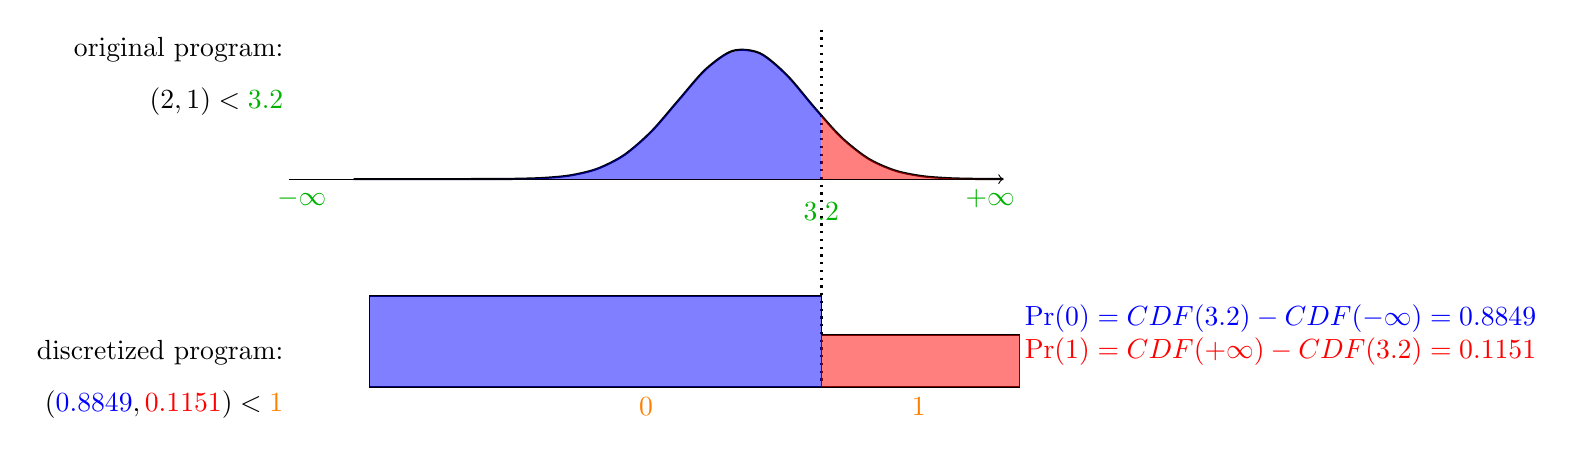
\begin{tikzpicture}[scale=1.1]

  % ===== BEGIN GRAPH REGION =====
  \begin{scope}[xshift=-2.5cm, scale=0.75]

  % Axes for Gaussian
  \draw[->] (-5,0) -- (6,0);
  \node[text=green!70!black] at (-4.8, -0.3) {$-\infty$};
  \node[text=green!70!black] at (5.8, -0.3) {$+\infty$};
  \node[text=green!70!black] at (3.2, -0.5) {3.2};

  % Gaussian curve: N(2,1)
  \draw[thick, domain=-4:6, smooth, variable=\x] 
    plot ({\x},{2*exp(-((\x-2)*(\x-2))/2)});

  % Vertical dotted line 
  \draw[dotted, thick] (3.2, 2.3) -- (3.2, -3.2);

  % Blue shading (left interval)
  \fill[blue, opacity=0.5] 
    (-4,0) -- plot[domain=-4:3.2] (\x,{2*exp(-((\x-2)*(\x-2))/2)}) -- (3.2,0) -- cycle;

  % Red shading (right interval)
  \fill[red, opacity=0.5] 
    (3.2,0) -- plot[domain=3.2:6] (\x,{2*exp(-((\x-2)*(\x-2))/2)}) -- (6,0) -- cycle;

  % Discrete distribution: 0 bar
  \draw (-3.75,-1.8) rectangle (3.2,-3.2);

  % Discrete distribution: 1 bar
  \draw (3.2,-2.4) rectangle (6.25,-3.2);

  % Fill colors
  \fill[blue, opacity=0.5] (-3.75,-1.8) rectangle (3.2,-3.2);
  \fill[red, opacity=0.5] (3.2,-2.4) rectangle (6.25,-3.2);

  % Labels
  \node[text=orange] at (0.5,-3.5) {0};
  \node[text=orange] at (4.7,-3.5) {1};

  \end{scope}
  % ===== END GRAPH REGION =====

  % Original program text
  \node[left] at (-6.2,1.5) {original program:};
  \node[left] at (-6.2,0.9) {$\gaussian(2,1) < \textcolor{green!70!black}{3.2}$};

  % Discretized program text
  \node[left] at (-6.2,-2.0) {discretized program:};
  \node[left] at (-6.2,-2.6) {$\discrete(\textcolor{blue}{0.8849}, \textcolor{red}{0.1151}) < \textcolor{orange}{1}$};

  % Probability equations
  \node[align=left] at (5.2,-1.8) {
  \textcolor{blue}{$\Pr(0) = CDF(3.2) - CDF(-\infty)= 0.8849$}\\
  \textcolor{red}{$\Pr(1) = CDF(+\infty) - CDF(3.2) = 0.1151$}
  };

  \end{tikzpicture}
  }
  \caption{Discretization of the original program $\gaussian(2,1) < 3.2$ into the semantically equivalent discretized program $\discrete(0.8849, 0.1151) < 1$. The blue and red shaded regions show how the cut at 3.2 partitions the continuous distribution into two intervals $(-\infty, 3.2)$ and $[3.2, +\infty)$, whose masses become the probabilities of outcomes $0$ and $1$, e.g. interval indices, in the discrete distribution.}
  \label{fig:cuts-gaussian}
\end{figure}

\iffalse
\begin{figure}
    \centering
    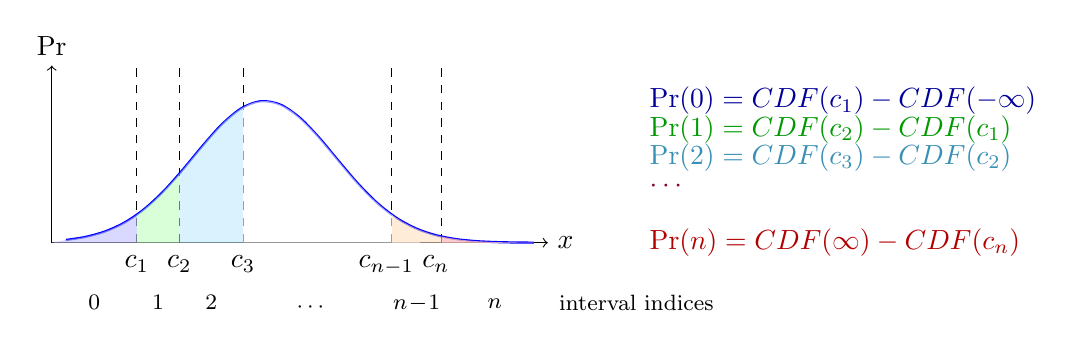
\begin{tikzpicture}[scale=0.9]
      % Axes
      \draw[->] (0,0) -- (7,0) node[right] {$x$};
      \draw[->] (0,0) -- (0,2.5) node[above] {$\Pr$};
    
      % Continuous distribution curve
      \draw[domain=0.2:6.8, smooth, variable=\x, thick, blue]
        plot ({\x}, {2*exp(-0.5*((\x-3)^2))});
    
      % Vertical cut lines with labels (shift c_{n-1} and c_n left slightly)
      \foreach \x/\label in {1.2/$c_1$, 1.8/$c_2$, 2.7/$c_3$, 4.8/{\hspace{-4pt}$c_{n-1}$}, 5.5/{\hspace{-4pt}$c_n$}} {
        \draw[dashed] (\x,0) -- (\x,2.5);
        \node[below] at (\x,-0.05) {\label};
    }
    
      % Shading intervals (different colors)
      \fill[blue!25, opacity=0.6] (0,0)
          -- plot[domain=0.2:1.2] ({\x}, {2*exp(-0.5*((\x-3)^2))})
          -- (1.2,0) -- cycle;
    \fill[green!25, opacity=0.6] (1.2,0)
          -- plot[domain=1.2:1.8] ({\x}, {2*exp(-0.5*((\x-3)^2))})
          -- (1.8,0) -- cycle;
      \fill[cyan!25, opacity=0.6] (1.8,0)
          -- plot[domain=1.8:2.7] ({\x}, {2*exp(-0.5*((\x-3)^2))})
          -- (2.7,0) -- cycle;
      \fill[white!25, opacity=0.6] (2.7,0)
          -- plot[domain=2.7:4.8] ({\x}, {2*exp(-0.5*((\x-3)^2))})
          -- (5.2,0) -- cycle;
      \fill[orange!25, opacity=0.6] (4.8,0)
            -- plot[domain=4.8:5.5] ({\x},{2*exp(-0.5*((\x-3)^2))})
            -- (5.5,0) -- cycle;
      \fill[red!25, opacity=0.8] (5.5,0)
            -- plot[domain=5.5:6.8] ({\x},{2*exp(-0.5*((\x-3)^2))})
            -- (6.8,0) -- cycle;

    % Interval number labels (shift n-1 and n left slightly)
    \node[below] at (0.6,-0.6) {\footnotesize $0$};
    \node[below] at (1.5,-0.6) {\footnotesize$1$};
    \node[below] at (2.25,-0.6) {\footnotesize$2$};
    \node[below] at (3.65,-0.7) {\footnotesize$\cdots$};
    \node[below] at (5.15,-0.6) {\footnotesize$n\!-\!1$};   % shifted 0.1 left
    \node[below] at (6.25,-0.65) {\footnotesize$n$};         % shifted 0.15 left
       \node[below] at (8.25,-0.6) {\footnotesize interval indices}; 
      % Color-matched probability annotations
      \node[right, text=blue!60!black]  at (8.3,2.0) {$\Pr(0) = \text{CDF}(c_1) - \text{CDF}(-\infty)$};
      \node[right, text=green!60!black]   at (8.3,1.6) {$\Pr(1) = \text{CDF}(c_2) - \text{CDF}(c_1)$};
      \node[right, text=cyan!70!black]at (8.3,1.2) {$\Pr(2) = \text{CDF}(c_3) - \text{CDF}(c_2)$};
      \node[right, text=purple!70!black]at (8.3,0.8) {$\cdots$};
      \node[right, text=red!70!black]   at (8.3,0.0) {$\Pr(n) = \text{CDF}(\infty) - \text{CDF}(c_n)$};
    
    \end{tikzpicture}
    \caption{Partitioning a continuous distribution by cuts $\clt{c_1}, \ldots, \clt{c_n}$ into intervals $(-\infty, c_1), [c_1,c_2), \ldots, [c_n, +\infty)$, with each interval assigned a discrete probability $\Pr(i)$ computed from CDF differences. Each interval represents a range of real values that is abstracted to a single discretized value labeled $0, 1, \ldots, n$. Note the resulting intervals may vary in width and need not be uniformly spaced. Given an expression of type $\floattype{B}{V}$, a finite value set $V$ maps the expression to the unique interval containing that value, whereas $V = \top$ yields a discrete distribution over all interval indices $i$, weighted by their probabilities $\Pr(i)$.}
    \label{fig:cuts-distr}
\end{figure}
\fi


\subsection{Branching on Multiple Continuous Variables}\label{sec:examples:2}

\noindent Let us now consider a more complex example with multiple continuous variables and conditionals:

\begin{lstlisting}[aboveskip=1em,belowskip=1em]
    let x = uniform(0, 1) in
    let y = uniform(0, 2) in
    if x < 0.5 then x < 0.2 else y < 0.1
\end{lstlisting}

\noindent In this program, the variable $x$ is drawn from \uniform(0, 1) and is compared against two different constants: $0.5$ and $0.2$. These two cuts $\clt{0.5}$ and $\clt{0.2}$ partition the real line $\R$ into three intervals: $(-\infty, 0.2)$, $[0.2, 0.5)$, and $[0.5, +\infty)$. Similarly, the variable $y$, drawn from \uniform(0, 2), is compared only with $0.1$. This single cut $\clt{0.1}$ partitions the real line $\R$ into two intervals, $(-\infty, 0.1)$ and $[0.1, +\infty)$.


This analysis is done by the type inference process, which collects all cuts for each continuous variable. For $x$, the type inference algorithm discovers the cuts $\clt{0.2}$ and $\clt{0.5}$, giving it the type \ft{<0.2,<0.5}. For $y$, it only finds $\clt{0.1}$, giving it the type \ft{<0.1}. This information is captured in the annotated program below (omitting the redundant types):

\begin{lstlisting}[aboveskip=1em,belowskip=1em,escapechar=!]
    let x = uniform(0, 1) : !{\ft{<0.2,<0.5}}! in
    let y = uniform(0, 2) : !{\ft{<0.1}}! in
    if x < (0.5 : !{\ftb{<0.2,<0.5}{0.5}}!) then
      x < (0.2 : !{\ftb{<0.2,<0.5}{0.2}}!)
    else
      y < (0.1 : !{\ftb{<0.1}{0.1}}!)
\end{lstlisting}


\Slice{} therefore discretizes $x$ into three outcomes \discrete(0.2, 0.3, 0.5) and $y$ into two outcomes \discrete(0.05, 0.95), where each probability is the measure of the original interval. Comparisons now operate over the integer indices of those intervals:

\begin{lstlisting}[aboveskip=1em,belowskip=1em]
    let x = discrete(0.2, 0.3, 0.5) in
    let y = discrete(0.05, 0.95) in
    if x < 2 then x < 1 else  y < 1
\end{lstlisting}

%Using \Dice{}, this yields the output \result{0.225}{0.775}.
The constant $0.5$ maps to index 2 for $x$ and 1 for $y$ because it lands in different partitions: $(-\infty,0.2)\cup[0.2,0.5)\cup[0.5,+\infty)$ for the first comparison, versus $(-\infty,0.5)\cup[0.5,+\infty)$ for the second. 

\iffalse
\subsection{Discretizing Float Constants}\label{sec:examples:3}
The example in Section~\ref{sec:examples:2} involves comparisons with literal constant right-hand sides (such as $e < 0.5$). 
\Slice{} does not require the comparison to have a syntactic constant right-hand or left-hand side. Instead, it analyzes the dataflow of the program to determine which constants are relevant, and how these constants are mapped to discrete indices.
Consider the program:

\begin{lstlisting}[aboveskip=1em,belowskip=1em,escapechar=!]
    let x = if flip() then 0.2 
            else if flip() then 2.5
            else 4.5 in 
    let y = 0.5 in x < y
\end{lstlisting}

This yields the annotated program after type inference:

\begin{lstlisting}[aboveskip=1em,belowskip=1em,escapechar=!]
    let x = if flip() then (0.2 : !{\ftb{<0.5}{0.2}}!)
            else (if flip() then (2.5 : !{\ftb{<0.5}{2.5}}!)
            else (4.5 : !{\ftb{<0.5}{4.5}}!) 
            : !{\ftb{<0.5}{2.5, 4.5}}!)
            : !{\ftb{<0.5}{0.2, 2.5, 4.5}}! in
    let y = 0.5 : !{\ftb{<0.5}{0.5}}! in x < y
\end{lstlisting}

Both $x$ and $y$ can only take on finitely many values --- a fact which is reflected by the value sets in the type annotations. By locating where each value in the value set falls relative to the cuts in the cut set, \Slice{} determines the corresponding interval index for each value. \codetype{\ftb{<0.5}{0.2}} corresponds to the index 0, and types \codetype{\ftb{<0.5}{2.5}}, \codetype{\ftb{<0.5}{4.5}}, and \codetype{\ftb{<0.5}{0.5}} all correspond to the index 1. The value sets in types \codetype{\ftb{<0.5}{0.2, 2.5, 4.5}} and \codetype{\ftb{<0.5}{2.5, 4.5}} arise from taking the union of the value sets from each prior conditional branch. This in turn yields the following discretized program:

\begin{lstlisting}[aboveskip=1em,belowskip=1em]
    let x = if flip() then 0
            else if flip() then 1
            else 1 in
    let y = 1
    x < y
\end{lstlisting}

Notice how both $2.5$ and $4.5$ are discretized to $1$, because for the purpose of comparing them to $y = 0.5$, these values are equivalent.

%Using \Dice{}, this yields the output \result{0.5}{0.5}.
\fi
\subsection{Control flow}\label{sec:examples:4}

Continuous values often flow through conditionals before being compared. The same discretization applies, as the following type-annotated program illustrates:

%\begin{lstlisting}[aboveskip=1em,belowskip=1em,escapechar=!]
%    let x = if flip() then uniform(0,2) 
%            else gaussian(0,1) in
%    let y = if 1.5 > x
%            then 1.8
%            else 0.3 in
%    x <= y
%\end{lstlisting}
\begin{lstlisting}[aboveskip=1em,belowskip=1em,escapechar=!]
    let x = if flip()
            then (uniform(0,2) : !{\ft{<=0.3,<1.5,<=1.8}}!)
            else (gaussian(0,1) : !{\ft{<=0.3,<1.5,<=1.8}}!)
            : !{\ft{<=0.3,<1.5,<=1.8}}! in
    let y = if (1.5 : !{\ftb{<=0.3,<1.5,<=1.8}{1.5}}!) > x
            then (1.8 : !{\ftb{<=0.3,<1.5,<=1.8}{1.8}}!)
            else (0.3 : !{\ftb{<=0.3,<1.5,<=1.8}{0.3}}!)
            : !{\ftb{<=0.3,<1.5,<=1.8}{0.3,1.8}}! in
    x <= y
\end{lstlisting}
\noindent \Slice{} propagates the cuts introduced in $y$ back to the samplings of $x$. Because the final comparison forces both sides to share cuts, every subexpression uses $\cleq{0.3}$, $\clt{1.5}$, and $\cleq{1.8}$, i.e.\ type \codetype{\ft{<=0.3,<1.5,<=1.8}}.



\noindent The resulting intervals are $(-\infty,0.3]$, $(0.3,1.5)$, $[1.5,1.8]$, and $(1.8,+\infty)$; the strict comparison excludes 1.5 from the second one. The guard in $y$ therefore reads indices 1, 2, or 0 coming from types \codetype{\ftb{<=0.3,<1.5,<=1.8}{1.5}}, \codetype{\ftb{<=0.3,<1.5,<=1.8}{1.8}}, and \codetype{\ftb{<=0.3,<1.5,<=1.8}{0.3}} respectively. Discretization yields:

\begin{lstlisting}[aboveskip=1em,belowskip=1em]
    let x = if flip() then
        discrete(0.15, 0.6, 0.15, 0.1)
      else
        discrete(0.617911, 0.315281, 0.0308769, 0.0359303) in
    let y = if 1 > x then 2 else 0 in
    x <= y
\end{lstlisting}

\noindent Each \discrete-expression lists the mass of those four intervals. For instance, \uniform(0,2) assigns $(0.15, 0.6, 0.15, 0.1)$.

\subsection{Discrete Latent Variable}\label{sec:examples:5}

Continuous distributions can have parameters that depend on discrete random choices. In this example, a Gaussian distribution's standard deviation is determined by a such a random choice:

\begin{lstlisting}[aboveskip=1em,belowskip=1em,escapechar=!]
    let x = if flip() then 0.5 else 1.5 in gaussian(0, x) < 0.5
\end{lstlisting}

\iffalse
\noindent %This example shows how discrete choices can affect the parameters of continuous distributions. 
The type-annotations reveal how the variable $x$ determines the standard deviation of the Gaussian:

\begin{lstlisting}[aboveskip=1em,belowskip=1em,escapechar=!]
    let x = if flip() then (0.5 : !{\ftb{<=0.5,<=1.5}{0.5}}!)
                      else (1.5 : !{\ftb{<=0.5,<=1.5}{1.5}}!)
             : !{\ftb{<=0.5,<=1.5}{0.5,1.5}}! in
            (gaussian(0, x) : !{\ft{<0.5}}!) < (0.5 : !{\ftb{<0.5}{0.5}}!)
\end{lstlisting}

\noindent Since the variable $x$ is later used as a parameter to the $\gaussian$ distribution, \Slice{} generates a separate case for each possible value that $x$ can take (namely 0.5 and 1.5). To support this, the type system uses non-strict inequalities in the cut sets, enabling these values to be mapped to integer indices starting from 0. Specifically, the value 0.5 corresponds to index 0 via the type \codetype{\ftb{<=0.5,<=1.5}{0.5}}, and 1.5 corresponds to 1 via \codetype{\ftb{<=0.5,<=1.5}{1.5}}. The resulting discretized program then branches on these values and instantiates the corresponding discrete distribution, depending on which standard deviation was selected by the initial flip.

\begin{lstlisting}[aboveskip=1em,belowskip=1em]
    let x = if flip() then 0 else 1 in
    (if x == 0 then  discrete(0.841345, 0.158655)
               else  discrete(0.630559, 0.369441)) < 1
\end{lstlisting}
%
\noindent
%Using \Dice{}, this yields the output \result{0.73595}{0.26405}.
\fi

\subsection{Conditioning}\label{sec:examples:6}

\Slice{} supports conditioning via $\observekw$. The program below (already type-annotated) computes $\Pr[x<0.2 \mid x<0.5]$ for $x \sim \uniform(0,1)$:

%\begin{lstlisting}[aboveskip=1em,belowskip=1em,escapechar=!]
%    let x = uniform(0.0, 1.0) in
%    let _ = observe (x < 0.5) in
%    x < 0.2
%\end{lstlisting}
%
%\noindent The type annotations show how observation points become cuts:

\begin{lstlisting}[aboveskip=1em,belowskip=1em,escapechar=!]
    let x = (uniform(0.0, 1.0) : !{\ft{<0.2,<0.5}}!) in
    let _ = observe (x < (0.5 : !{\ftb{<0.2,<0.5}{0.5}}!)) in
    x < (0.2 : !{\ftb{<0.2,<0.5}{0.2}}!)
\end{lstlisting}

\noindent Discretization again replaces reals by interval indices:

\begin{lstlisting}[aboveskip=1em,belowskip=1em]
    let x = discrete(0.2, 0.3, 0.5) in
    let _ = observe (x < 2) in
    x < 1
\end{lstlisting}

\noindent Observation $x<2$ eliminates the discrete state corresponding to the original interval $[0.5,+\infty)$, mirroring the conditioning on $x<0.5$.

Exact equalities can be encoded with $\observekw\; (x \leq c \mathrel{\&\&} x \geq c)$. Measure-zero observations remain delicate~\cite{Jacobs2021ParadoxesProbProg}; our semantics handles them by recording observation failure mass instead of renormalizing, so discretization preserves an even stronger equivalence. Scoring semantics for true measure-zero events are out of scope; users should instead approximate them with narrow intervals.
